%----------------------------------------------------------------------------------------
%    PACKAGES AND THEMES
%----------------------------------------------------------------------------------------

\documentclass[aspectratio=169,xcolor=dvipsnames]{beamer}
\usetheme{SimplePlus}

\usepackage{hyperref}
\usepackage{graphicx} % Allows including images
\usepackage{booktabs} % Allows the use of \toprule, \midrule and \bottomrule in tables

\usepackage[caption=false]{subfig}

\usepackage{tikz}
\usetikzlibrary{positioning}

\usepackage{pgfplots}
\usepgfplotslibrary{groupplots}
\pgfplotsset{compat=1.18}

\usepackage{xspace}
\newcommand{\modelministral}{Ministral-8B\xspace}
\newcommand{\modelalpaca}{Alpaca-7B\xspace}
\newcommand{\modeldeepseek}{R1-Distill-8B\xspace}

%----------------------------------------------------------------------------------------
%    TITLE PAGE
%----------------------------------------------------------------------------------------

\title{Knowledge Graph Completion}
\subtitle{Subtitle}

\author{Eddie Groh \and Mochamad Ardiansyah Nurgaha \and Sriraam Appakutti Palani \and William Liaw}

\institute[Team: AWESome]
{
    Mehwish ALAM\\
    Associate Professor
    \and
    Language Models and Structured Data\\
}
\date{\today}

%----------------------------------------------------------------------------------------
%    PRESENTATION SLIDES
%----------------------------------------------------------------------------------------

\begin{document}

\begin{frame}
    % Print the title page as the first slide
    \titlepage
\end{frame}

% \begin{frame}{Overview}
%     \tableofcontents
% \end{frame}

%------------------------------------------------
\section{Problem Statement \& Background}
%------------------------------------------------
\begin{frame}{Problem Statement}
    \begin{itemize}
        \item Knowledge Graph Completion (KGC) aims to infer missing facts in a knowledge graph (KG).
        \item A KG is defined as $G = (E, R, T)$ where:
              \begin{itemize}
                  \item $E$ is the set of entities
                  \item $R$ is the set of relations
                  \item $T \subseteq E \times R \times E$ represents valid triples
              \end{itemize}
        \item Two fundamental tasks:
              \begin{itemize}
                  \item \textbf{Link Prediction}: Predicting missing entities.
                  \item \textbf{Triple Classification}: Determining validity of a triple.
              \end{itemize}
    \end{itemize}
\end{frame}

\begin{frame}{Background}
    \begin{itemize}
        \item Early approaches used embedding-based models:
              \begin{itemize}
                  \item TransE, DistMult, ComplEx.
              \end{itemize}
        \item Large Language Models (LLMs) improve KGC by leveraging:
              \begin{itemize}
                  \item In-context learning.
                  \item Instruction tuning.
              \end{itemize}
        \item Two main strategies:
              \begin{itemize}
                  \item \textbf{Prompt-Based Methods} (e.g., KICGPT).
                  \item \textbf{Fine-Tuning-Based Methods} (e.g., KoPA).
              \end{itemize}
    \end{itemize}
\end{frame}

%------------------------------------------------
\section{Methodology}
%------------------------------------------------
\begin{frame}{KICGPT: Prompt-Based Link Prediction}
    \begin{itemize}
        \item Uses retrieval and ranking for entity prediction.
        \item Steps:
              \begin{itemize}
                  \item Retrieve candidate entities.
                  \item Use Knowledge Prompts to refine ranking.
                  \item Final ranking by LLM-based reranking.
              \end{itemize}
    \end{itemize}
    \begin{figure}[h]
        \centering
        \includegraphics[width=0.8\linewidth]{images/KICGPTarchitecture.png}
        \caption{KICGPT Architecture}
    \end{figure}
\end{frame}


\begin{frame}{KoPA: Fine-Tuning-Based Triple Classification}
    \begin{itemize}
        \item Uses Knowledge Prefix Adapter (KPA) to integrate KG structure.
        \item Embeddings guide LLM reasoning.
        \item Fine-tuned LLM predicts validity of triples.
    \end{itemize}
    \begin{figure}[h]
        \centering
        \includegraphics[width=0.8\linewidth]{images/KoPAarchitecture.png}
        \caption{KoPA Architecture}
    \end{figure}
\end{frame}


%------------------------------------------------
\section{Experiments \& Discussion}
%------------------------------------------------
\begin{frame}{Experiments}
    \begin{itemize}
        \item Datasets: WN18RR and CoDeX-S.
        \item Evaluation metrics:
              \begin{itemize}
                  \item Mean Reciprocal Rank (MRR), Hits@1, Hits@3, Hits@10.
              \end{itemize}
        \item Compared models: Alpaca-7B, Ministral-8B, R1-Distill-8B.
    \end{itemize}
    \begin{table}[h]
        \centering
        \begin{tabular}{l c c c c c}
            \toprule
            \textbf{Dataset} & \textbf{\# Entities} & \textbf{\# Relations} & \textbf{\# train} & \textbf{\# valid} & \textbf{\# test} \\
            \midrule
            WN18RR           & 40,943               & 11                    & 86,835            & 3,034             & 3,134            \\
            CoDeX-S          & 2,034                & 42                    & 32,888            & 3,654             & 3,654            \\
            \bottomrule
        \end{tabular}
        \caption{Statistics of the datasets used in our experiments.}
        \label{tab:datasets}
    \end{table}
\end{frame}

\begin{frame}{Plots}
    \begin{columns}[c] % The "c" option specifies centered vertical alignment while the "t" option is used for top vertical alignment

        \column{.45\textwidth} % Left column and width
        \begin{figure}[ht]
            \centering
            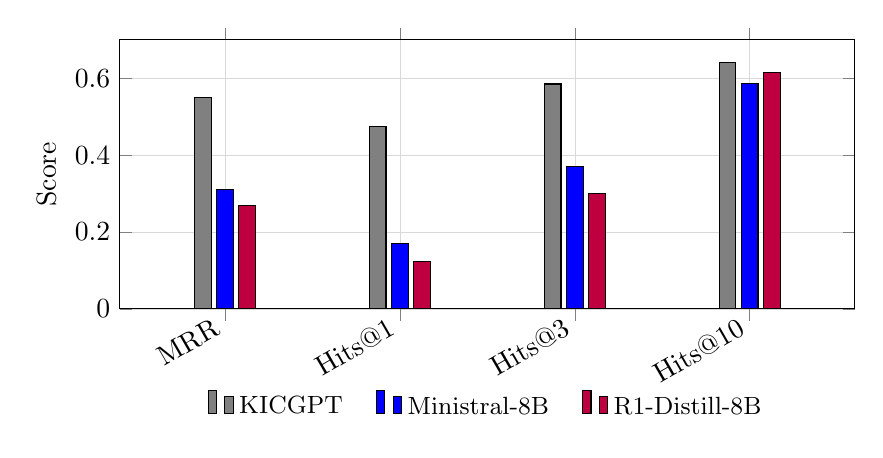
\begin{tikzpicture}
                \begin{axis}[
                        ybar,
                        bar width=6pt,
                        symbolic x coords={MRR, Hits@1, Hits@3, Hits@10},
                        xtick=data,
                        xticklabel style={rotate=30, anchor=east},
                        ymin=0,
                        ymax=0.7,
                        ylabel={Score},
                        width=0.9\textwidth,
                        height=5cm,
                        grid=both,
                        major grid style={line width=.2pt, draw=gray!30},
                        minor grid style={draw=gray!10},
                        enlarge x limits=0.2,
                        % Legend placed below with spacing:
                        legend style={
                                at={(0.5,-0.28)},
                                anchor=north,
                                /tikz/every even column/.append style={column sep=10pt},
                                legend columns=3,
                                draw=none, % Remove box
                                fill=none,
                                font=\small
                            }
                    ]

                    % Bars
                    \addplot[fill=gray]   coordinates {(MRR,0.549)  (Hits@1,0.474)  (Hits@3,0.585)  (Hits@10,0.641)};
                    \addlegendentry{KICGPT}
                    \addplot[fill=blue]   coordinates {(MRR,0.3112) (Hits@1,0.1707) (Hits@3,0.3711) (Hits@10,0.5862)};
                    \addlegendentry{\modelministral}
                    \addplot[fill=purple] coordinates {(MRR,0.2700) (Hits@1,0.1233) (Hits@3,0.2994) (Hits@10,0.6145)};
                    \addlegendentry{\modeldeepseek}

                \end{axis}
            \end{tikzpicture}
            \caption{Link Ordering Evaluation Metrics}
            \label{fig:link_ordering}
        \end{figure}

        \column{.45\textwidth} % Right column and width
        \begin{figure}[ht]
            \centering
            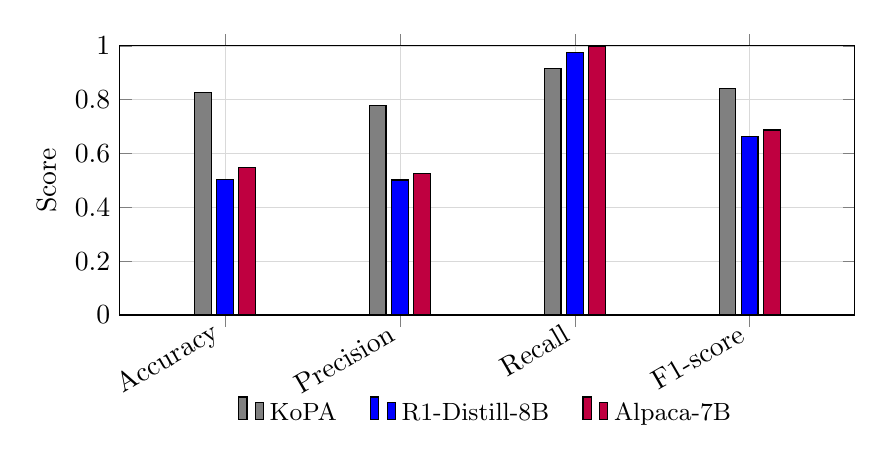
\begin{tikzpicture}
                \begin{axis}[
                        ybar,
                        bar width=6pt,
                        symbolic x coords={Accuracy, Precision, Recall, F1-score},
                        xtick=data,
                        xticklabel style={rotate=30, anchor=east},
                        ymin=0,
                        ymax=1,
                        ylabel={Score},
                        width=0.9\textwidth,
                        height=5cm,
                        grid=both,
                        major grid style={line width=.2pt, draw=gray!30},
                        minor grid style={draw=gray!10},
                        enlarge x limits=0.2,
                        legend style={
                                at={(0.5,-0.28)},
                                anchor=north,
                                /tikz/every even column/.append style={column sep=10pt},
                                legend columns=3,
                                draw=none,
                                fill=none,
                                font=\small
                            }
                    ]

                    % Bars
                    \addplot[fill=gray]   coordinates {(Accuracy,0.8274)  (Precision,0.7791)  (Recall,0.9141)  (F1-score,0.8411)};
                    \addlegendentry{KoPA}

                    \addplot[fill=blue]   coordinates {(Accuracy,0.5027) (Precision,0.5014) (Recall,0.9759) (F1-score,0.6625)};
                    \addlegendentry{\modeldeepseek}

                    \addplot[fill=purple] coordinates {(Accuracy,0.5465) (Precision,0.5245) (Recall,0.9962) (F1-score,0.6872)};
                    \addlegendentry{\modelalpaca}
                \end{axis}
            \end{tikzpicture}
            \caption{CoDeX Performance Evaluation Metrics}
            \label{fig:codex_evaluation}
        \end{figure}

    \end{columns}
\end{frame}

\begin{frame}{Plots}
    \begin{figure}
        \centering
        \begin{tikzpicture}
            % Group plot configuration
            \begin{groupplot}[
                    group style={
                            group size=3 by 1,       % 3 plots in 1 row
                            horizontal sep=0.3cm     % Adjust spacing between plots
                        },
                    width=0.3\textwidth,         % Maximized plot width
                    ymode=log,                   % Log-scale y-axis for ALL plots
                    xmin=0, xmax=3,              % Unified x-axis range
                    ymin=1e-3, ymax=1,           % Unified y-axis range across all plots
                    xlabel=Epoch,
                    xtick distance=0.5,          % Uniform tick spacing
                    ytick distance=10,           % Log-scale tick separation
                    minor y tick num=9,          % Minor tick marks for readability
                ]

                %------------- Plot (a) Alpaca -----------------
                \nextgroupplot[
                    title=\modelalpaca,
                    % Hide y-axis labels for alignment
                    ylabel=Loss
                ]
                \addplot[smooth, thick, blue]
                table[x=epoch, y=loss, col sep=space]
                    {images/raw-data/lora-Llama-2-7b-alpaca-cleaned-finetune.dat};

                \addplot[smooth, thick, cyan, dashed]
                table[x=epoch, y=grad-norm, col sep=space]
                    {images/raw-data/lora-Llama-2-7b-alpaca-cleaned-finetune.dat};


                %------------- Plot (b) DeepSeek ---------------
                \nextgroupplot[
                    title=\modeldeepseek,
                    yticklabels={,,}
                ]
                \addplot[smooth, thick, purple]
                table[x=epoch, y=loss, col sep=space]
                    {images/raw-data/lora-DeepSeek-R1-Distill-Llama-8B-finetune.dat};

                \addplot[smooth, thick, violet, dashed]
                table[x=epoch, y=grad-norm, col sep=space]
                    {images/raw-data/lora-DeepSeek-R1-Distill-Llama-8B-finetune.dat};

                %------------- Plot (c) Loss Comparison -------------
                \nextgroupplot[
                    title=Loss Comparison,
                    yticklabels={,,}   % Hide y-axis tick labels for uniform look
                ]
                \addplot[smooth, thick, purple]
                table[x=epoch, y=loss, col sep=space]
                    {images/raw-data/lora-DeepSeek-R1-Distill-Llama-8B-finetune.dat};

                \addplot[smooth, thick, blue]
                table[x=epoch, y=loss, col sep=space]
                    {images/raw-data/lora-Llama-2-7b-alpaca-cleaned-finetune.dat};

            \end{groupplot}
        \end{tikzpicture}

        % Description of colors with more spacing in legend
        \vspace{0.2cm}
        {\centering
            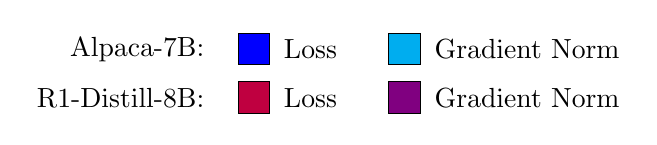
\begin{tikzpicture}
                \node[draw, fill=blue, minimum width=0.4cm, minimum height=0.4cm] (A) {};
                \node[left=0.3cm of A] {\modelalpaca:};
                \node[right=0.05cm of A] {Loss};

                \node[draw, fill=cyan, minimum width=0.4cm, minimum height=0.4cm, right=1.5cm of A] (B) {};
                \node[right=0.05cm of B] {Gradient Norm};

                \node[draw, fill=purple, minimum width=0.4cm, minimum height=0.4cm, below=0.2cm of A] (C) {};
                \node[left=0.3cm of C] {\modeldeepseek:};
                \node[right=0.05cm of C] {Loss};

                \node[draw, fill=violet, minimum width=0.4cm, minimum height=0.4cm, right=1.5cm of C] (D) {};
                \node[right=0.05cm of D] {Gradient Norm};
            \end{tikzpicture}
        }

        \caption{Fine-tuning of \modelalpaca and \modeldeepseek. Loss and gradient norm trends are shown separately for each model, along with a comparison of both losses. Figure and results from our work.}
        \label{fig:training_comparison}
    \end{figure}
\end{frame}

\begin{frame}{Discussion}
    \begin{itemize}
        \item KICGPT improves ranking by leveraging structured prompts.
              \begin{itemize}
                  \item ChatGPT outperforms \modeldeepseek and \modelministral due to better reranking heuristics.
              \end{itemize}
        \item KoPA integrates KG embeddings effectively for classification.
    \end{itemize}
\end{frame}

%------------------------------------------------
\section{Conclusion}
%------------------------------------------------
\begin{frame}{Conclusion}
    TBD
\end{frame}

% TEMPLATE STARTS HERE...

%------------------------------------------------
\section{First Section}
%------------------------------------------------

\begin{frame}{Bullet Points}
    \begin{itemize}
        \item Lorem ipsum dolor sit amet, consectetur adipiscing elit
        \item Aliquam blandit faucibus nisi, sit amet dapibus enim tempus eu
        \item Nulla commodo, erat quis gravida posuere, elit lacus lobortis est, quis porttitor odio mauris at libero
        \item Nam cursus est eget velit posuere pellentesque
        \item Vestibulum faucibus velit a augue condimentum quis convallis nulla gravida
    \end{itemize}
\end{frame}

%------------------------------------------------

\begin{frame}{Blocks of Highlighted Text}
    In this slide, some important text will be \alert{highlighted} because it's important. Please, don't abuse it.

    \begin{block}{Block}
        Sample text
    \end{block}

    \begin{alertblock}{Alertblock}
        Sample text in red box
    \end{alertblock}

    \begin{examples}
        Sample text in green box. The title of the block is ``Examples".
    \end{examples}
\end{frame}

%------------------------------------------------

\begin{frame}{Multiple Columns}
    \begin{columns}[c] % The "c" option specifies centered vertical alignment while the "t" option is used for top vertical alignment

        \column{.45\textwidth} % Left column and width
        \textbf{Heading}
        \begin{enumerate}
            \item Statement
            \item Explanation
            \item Example
        \end{enumerate}

        \column{.45\textwidth} % Right column and width
        Lorem ipsum dolor sit amet, consectetur adipiscing elit. Integer lectus nisl, ultricies in feugiat rutrum, porttitor sit amet augue. Aliquam ut tortor mauris. Sed volutpat ante purus, quis accumsan dolor.

    \end{columns}
\end{frame}

%------------------------------------------------
\section{Second Section}
%------------------------------------------------

\begin{frame}{Theorem}
    \begin{theorem}[Mass--energy equivalence]
        $E = mc^2$
    \end{theorem}
\end{frame}

\begin{frame}[fragile] % Need to use the fragile option when verbatim is used in the slide
    \frametitle{Citation}
    An example of the \verb|\cite| command to cite within the presentation:\\~

    This statement requires citation \cite{p1}.
\end{frame}

%------------------------------------------------

\begin{frame}{References}
    \footnotesize
    \bibliography{reference.bib}
    \bibliographystyle{apalike}
\end{frame}

%----------------------------------------------------------------------------------------

\end{document}
